% Compile with: pdflatex DataSense-Project-Documentation.tex (run twice for TOC)
% Or use Overleaf: upload this file and compile.

\documentclass[11pt,a4paper]{article}
\usepackage[utf8]{inputenc}
\usepackage[T1]{fontenc}
\usepackage{lmodern}
\usepackage[margin=2.5cm]{geometry}
\usepackage{graphicx}
\usepackage{booktabs}
\usepackage{longtable}
\usepackage{array}
\usepackage{hyperref}
\usepackage{xcolor}
\usepackage{listings}
\usepackage{enumitem}
\usepackage{tikz}
\usetikzlibrary{shapes.geometric, arrows.meta, positioning}

\hypersetup{
  colorlinks=true,
  linkcolor=blue!60!black,
  urlcolor=blue!70!black,
  citecolor=blue!60!black
}

\lstset{
  basicstyle=\ttfamily\small,
  breaklines=true,
  frame=single,
  backgroundcolor=\color{gray!8},
  columns=fullflexible
}

\title{\textbf{DataSense}\\[0.4em]
\large Technical Documentation --- Chat Layer for Government Open Data}
\author{Mindcase Intern Project}
\date{\today}

\begin{document}
\maketitle
\tableofcontents
\newpage

%==============================================================================
\section{Executive Summary}
%==============================================================================

\textbf{DataSense} is a web application that lets users ask natural-language questions about Indian government datasets published on \textbf{data.gov.in}. The system:

\begin{enumerate}[noitemsep]
  \item Fetches live rows from the selected dataset using the official data.gov.in API.
  \item Injects that data into a large language model (LLM) prompt on the \textbf{server}.
  \item Streams an AI-generated answer back to the browser in Markdown format.
\end{enumerate}

The default datasets are \textbf{Census 2011} tables (Primary Census Abstract, population by age/sex, literacy and workers). API keys for data.gov.in and Groq never leave the server.

%==============================================================================
\section{Problem Statement \& Solution}
%==============================================================================

\subsection{Problem}
Government data is available via APIs, but non-technical users cannot easily query it. They need a conversational interface grounded in real data, not hallucinated numbers.

\subsection{Solution}
A \textbf{Retrieval-augmented style} chat flow: for each user question, the backend loads a sample of records from data.gov.in, attaches them to the LLM context, and instructs the model to answer only from that JSON sample.

%==============================================================================
\section{Technology Stack}
%==============================================================================

\begin{table}[h]
\centering
\caption{Core technologies}
\begin{tabular}{@{}llp{7.5cm}@{}}
\toprule
\textbf{Layer} & \textbf{Technology} & \textbf{Role} \\
\midrule
Framework & Next.js 16 (App Router) & Full-stack React framework; API routes + UI \\
Language & TypeScript 5 & Type safety across frontend and backend \\
UI library & React 19 & Component-based user interface \\
Styling & Tailwind CSS 4 & Utility-first CSS; dark/light themes \\
Animation & Framer Motion 12 & Sidebar, messages, micro-interactions \\
Icons & Lucide React & Consistent icon set \\
Markdown & react-markdown + remark-gfm & Render AI replies (tables, lists, code) \\
Toasts & Sonner & Error and status notifications \\
Validation & Zod 4 & Server environment variable validation \\
Government data & data.gov.in REST API & Live dataset rows (JSON) \\
LLM & Groq API & Model: \texttt{openai/gpt-oss-120b} (streaming) \\
Fonts & Geist (next/font) & Typography \\
Linting & ESLint + eslint-config-next & Code quality \\
\bottomrule
\end{tabular}
\end{table}

\subsection{Why this stack?}
\begin{itemize}[noitemsep]
  \item \textbf{Next.js}: Single repo for UI and secure API routes; keys stay on server.
  \item \textbf{TypeScript}: Easier maintenance and onboarding for teams.
  \item \textbf{Groq}: Fast inference with OpenAI-compatible streaming API.
  \item \textbf{Tailwind}: Rapid UI iteration matching modern chat products.
\end{itemize}

%==============================================================================
\section{High-Level Architecture}
%==============================================================================

\begin{figure}[h]
\centering
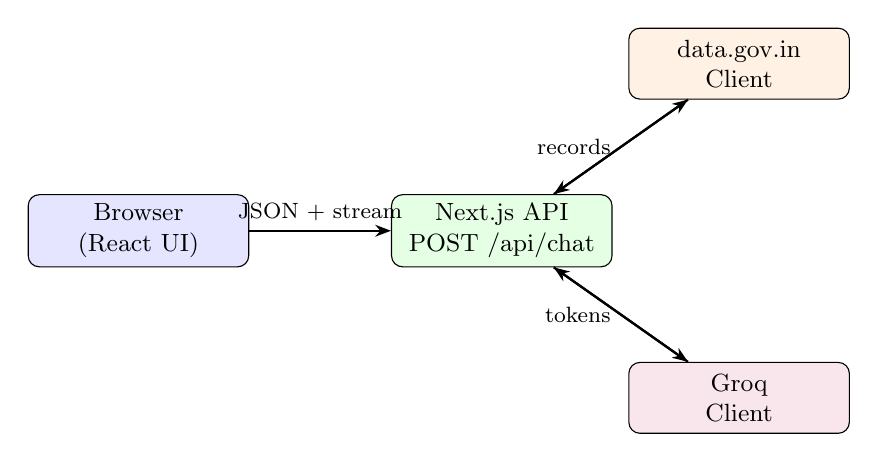
\begin{tikzpicture}[
  node distance=1.1cm and 1.8cm,
  box/.style={draw, rounded corners, minimum width=2.8cm, minimum height=0.9cm, align=center, font=\small},
  arr/.style={-{Stealth[length=2mm]}, thick}
]
  \node[box, fill=blue!10] (browser) {Browser\\(React UI)};
  \node[box, fill=green!10, right=of browser] (api) {Next.js API\\POST /api/chat};
  \node[box, fill=orange!10, above right=1.2cm and 0.2cm of api] (dg) {data.gov.in\\Client};
  \node[box, fill=purple!10, below right=1.2cm and 0.2cm of api] (groq) {Groq\\Client};
  \draw[arr] (browser) -- node[above, font=\footnotesize]{JSON + stream} (api);
  \draw[arr] (api) -- (dg);
  \draw[arr] (api) -- (groq);
  \draw[arr] (dg) -- node[left, font=\footnotesize]{records} (api);
  \draw[arr] (groq) -- node[left, font=\footnotesize]{tokens} (api);
\end{tikzpicture}
\caption{Request flow for one chat message}
\end{figure}

\subsection{Step-by-step (one user question)}
\begin{enumerate}
  \item User types a question and clicks Send.
  \item \texttt{useChat} hook sends \texttt{POST /api/chat} with \texttt{message}, \texttt{datasetId}, and recent \texttt{history}.
  \item \texttt{chat-service.ts} resolves the dataset from \texttt{registry.ts} and calls \texttt{fetchDataGovResource()}.
  \item Up to 50 rows (configurable) are trimmed to fit the prompt budget.
  \item \texttt{prompts.ts} builds a system prompt naming the dataset and embedding the JSON sample.
  \item \texttt{groq/client.ts} streams completion tokens; the API route pipes them to the browser as \texttt{text/plain}.
  \item \texttt{useChat} appends tokens to the assistant message; \texttt{MarkdownMessage} renders the result.
\end{enumerate}

%==============================================================================
\section{Repository Layout}
%==============================================================================

The project root is \texttt{Chat\_Layer\_For\_Gov\_Data/}. All application code lives in the \texttt{datasense/} subdirectory.

\begin{lstlisting}
Chat_Layer_For_Gov_Data/
  datasense/                    # Main Next.js application
    docs/                         # Documentation (this file)
    public/                       # Static assets
    scripts/                      # Utility scripts (dev/ops)
    src/
      app/                        # Next.js App Router (pages + API)
      components/                 # React UI components
      hooks/                      # Client-side React hooks
      lib/                        # Shared business logic (server + types)
    .env.example                  # Template for secrets (committed)
    .env.local                    # Real API keys (NOT committed)
    package.json                  # Dependencies and npm scripts
\end{lstlisting}

%==============================================================================
\section{File-by-File Reference}
%==============================================================================

\subsection{Configuration \& root files}

\begin{longtable}{@{}p{4.2cm}p{9.8cm}@{}}
\toprule
\textbf{File} & \textbf{Purpose} \\
\midrule
\endhead
\texttt{package.json} & Lists dependencies (Next, React, Groq integration libs) and scripts: \texttt{dev}, \texttt{build}, \texttt{start}, \texttt{lint}. \\
\texttt{package-lock.json} & Locked dependency versions for reproducible installs. \\
\texttt{tsconfig.json} & TypeScript compiler options; path alias \texttt{@/*} $\rightarrow$ \texttt{src/*}. \\
\texttt{next.config.ts} & Next.js configuration (currently minimal). \\
\texttt{next-env.d.ts} & Auto-generated Next.js TypeScript references. \\
\texttt{postcss.config.mjs} & PostCSS pipeline for Tailwind CSS v4. \\
\texttt{eslint.config.mjs} & ESLint rules (Next.js recommended). \\
\texttt{.env.example} & Documents all environment variables; safe to commit. \\
\texttt{.env.local} & Actual API keys and overrides; \textbf{gitignored}. \\
\texttt{README.md} & Quick start guide for developers. \\
\texttt{AGENTS.md}, \texttt{CLAUDE.md} & AI assistant hints for this repo (optional). \\
\bottomrule
\end{longtable}

\subsection{\texttt{public/} --- static assets}

\begin{longtable}{@{}p{4.2cm}p{9.8cm}@{}}
\toprule
\textbf{File} & \textbf{Purpose} \\
\midrule
\endhead
\texttt{public/*.svg} & Default Next.js placeholder SVGs. \\
\texttt{src/app/favicon.ico} & Browser tab icon (also referenced as logo in sidebar). \\
\bottomrule
\end{longtable}

\subsection{\texttt{scripts/}}

\begin{longtable}{@{}p{4.2cm}p{9.8cm}@{}}
\toprule
\textbf{File} & \textbf{Purpose} \\
\midrule
\endhead
\texttt{find-census-resource.mjs} & Developer utility: scrapes a data.gov.in resource page for UUIDs and tests which IDs return live API data. Used to configure Census 2011 resources. \\
\bottomrule
\end{longtable}

\subsection{\texttt{src/app/} --- routes (Next.js App Router)}

\begin{longtable}{@{}p{4.2cm}p{9.8cm}@{}}
\toprule
\textbf{File} & \textbf{Purpose} \\
\midrule
\endhead
\texttt{layout.tsx} & Root HTML shell: fonts (Geist), metadata, wraps app in \texttt{AppProviders}. \\
\texttt{page.tsx} & Home page; renders \texttt{DataSenseApp} (main UI). \\
\texttt{globals.css} & Global CSS, Tailwind imports, theme variables. \\
\texttt{api/chat/route.ts} & \textbf{Core API.} POST handler: validates body, runs \texttt{runDatasetChat()}, returns streaming text or JSON error. \\
\texttt{api/datasets/route.ts} & GET handler: returns public dataset metadata (labels, descriptions) for the UI---no secrets. \\
\bottomrule
\end{longtable}

\subsection{\texttt{src/components/datasense/} --- UI}

\begin{longtable}{@{}p{4.2cm}p{9.8cm}@{}}
\toprule
\textbf{File} & \textbf{Purpose} \\
\midrule
\endhead
\texttt{DataSenseApp.tsx} & Main layout: sidebar, chat area, mobile drawer, keyboard shortcuts (Ctrl+K search, Ctrl+B sidebar). Owns \texttt{datasetId} state. \\
\texttt{Sidebar.tsx} & Collapsible navigation: new chat, search, recent threads (demo list), user profile menu (settings, theme, dataset picker, help, logout). \\
\texttt{WelcomeHero.tsx} & Empty-state welcome screen before first message. \\
\texttt{MessageList.tsx} & Scrollable list of chat messages. \\
\texttt{MessageBubble.tsx} & Single message bubble (user vs assistant, streaming skeleton, error styling). \\
\texttt{MarkdownMessage.tsx} & Renders assistant Markdown (GFM tables, code blocks). \\
\texttt{ChatInput.tsx} & Text area, send button, shows active dataset label, attach/voice placeholders. \\
\texttt{SearchChatsDialog.tsx} & Modal to search demo chat thread titles. \\
\texttt{BackgroundBlobs.tsx} & Decorative gradient blobs behind the UI. \\
\texttt{ui/Skeleton.tsx} & Loading placeholder lines while AI streams. \\
\bottomrule
\end{longtable}

\subsection{\texttt{src/components/providers/}}

\begin{longtable}{@{}p{4.2cm}p{9.8cm}@{}}
\toprule
\textbf{File} & \textbf{Purpose} \\
\midrule
\endhead
\texttt{AppProviders.tsx} & Wraps children with \texttt{ThemeProvider} and Sonner \texttt{Toaster}. \\
\texttt{ThemeProvider.tsx} & Dark/light theme context; persists preference in \texttt{localStorage}. \\
\bottomrule
\end{longtable}

\subsection{\texttt{src/hooks/}}

\begin{longtable}{@{}p{4.2cm}p{9.8cm}@{}}
\toprule
\textbf{File} & \textbf{Purpose} \\
\midrule
\endhead
\texttt{useChat.ts} & Client chat state: messages array, \texttt{sendMessage}, \texttt{reset}, streaming fetch to \texttt{/api/chat}, error handling and rate-limit toasts. \\
\bottomrule
\end{longtable}

\subsection{\texttt{src/lib/} --- business logic}

\begin{longtable}{@{}p{4.2cm}p{9.8cm}@{}}
\toprule
\textbf{File} & \textbf{Purpose} \\
\midrule
\endhead
\texttt{env.ts} & \textbf{Server only.} Validates \texttt{process.env} with Zod (API keys, limits, model name). \\
\texttt{errors.ts} & \texttt{AppError} class with HTTP status and error codes for API responses. \\
\texttt{utils.ts} & \texttt{cn()} helper: merges Tailwind class names (\texttt{clsx} + \texttt{tailwind-merge}). \\
\texttt{chatThreads.ts} & Static demo list of ``recent'' chat titles in the sidebar. \\
\texttt{types/chat.ts} & Shared TypeScript types for API request/response bodies. \\
\midrule
\texttt{datasets/types.ts} & \texttt{DatasetId} and \texttt{DatasetConfig} types. \\
\texttt{datasets/registry.ts} & Maps sidebar keys (\texttt{sales}, \texttt{crm}, \texttt{ops}) to Census 2011 resource UUIDs on data.gov.in. \\
\texttt{datasets/constants.ts} & Client-safe dataset labels for sidebar (no secrets). \\
\midrule
\texttt{data-gov-in/types.ts} & Types for API records and fetch results. \\
\texttt{data-gov-in/client.ts} & Fetches JSON from data.gov.in (primary URL + fallback), normalizes response. \\
\midrule
\texttt{groq/errors.ts} & Rate-limit detection, retry delay parsing, user-facing messages. \\
\texttt{groq/client.ts} & Calls Groq chat completions with streaming; retries on HTTP 429. \\
\midrule
\texttt{ai/prompts.ts} & Builds the system prompt (dataset metadata + JSON sample + rules). \\
\texttt{ai/chat-service.ts} & Orchestrator: load data $\rightarrow$ trim context $\rightarrow$ call Groq stream. \\
\bottomrule
\end{longtable}

%==============================================================================
\section{Dataset Configuration (Census 2011)}
%==============================================================================

Internal sidebar keys are historical (\texttt{sales}, \texttt{crm}, \texttt{ops}) but map to Census APIs:

\begin{table}[h]
\centering
\begin{tabular}{@{}lll@{}}
\toprule
\textbf{Key} & \textbf{UI label} & \textbf{data.gov.in resource UUID} \\
\midrule
\texttt{sales} & Primary Census Abstract 2011 & \texttt{0764657f-00ec-4c6b-9ece-2d7b8a7401fa} \\
\texttt{crm} & Population by age \& sex, 2011 & \texttt{3fac8061-9b36-418d-a5d5-7cedd300c942} \\
\texttt{ops} & Literacy \& workers (PCA focus) & \texttt{0764657f-00ec-4c6b-9ece-2d7b8a7401fa} \\
\bottomrule
\end{tabular}
\caption{Default dataset mapping (\texttt{registry.ts})}
\end{table}

Override any ID in \texttt{.env.local} using \texttt{DATA\_GOV\_RESOURCE\_SALES}, etc.

%==============================================================================
\section{Environment Variables}
%==============================================================================

\begin{longtable}{@{}p{4.5cm}p{9.5cm}@{}}
\toprule
\textbf{Variable} & \textbf{Description} \\
\midrule
\endhead
\texttt{DATA\_GOV\_IN\_API\_KEY} & API key from data.gov.in (required). \\
\texttt{DATA\_GOV\_IN\_BASE\_URL} & Primary API base (default: \texttt{api.data.gov.in/resource}). \\
\texttt{DATA\_GOV\_IN\_FALLBACK\_URL} & Legacy datastore endpoint if primary fails. \\
\texttt{DATA\_GOV\_IN\_FETCH\_LIMIT} & Max rows fetched per question (default 50). \\
\texttt{DATA\_GOV\_IN\_TIMEOUT\_MS} & HTTP timeout for government API (default 60000). \\
\texttt{DATA\_GOV\_RESOURCE\_*} & Optional per-dataset resource UUID overrides. \\
\texttt{GROQ\_API\_KEY} & Groq API key (required). \\
\texttt{GROQ\_MODEL} & Model id (default: \texttt{openai/gpt-oss-120b}). \\
\texttt{GROQ\_MAX\_COMPLETION\_TOKENS} & Max tokens in AI reply (default 2048). \\
\texttt{GROQ\_TEMPERATURE} & Sampling temperature (default 0.3). \\
\texttt{GROQ\_RATE\_LIMIT\_MAX\_RETRIES} & Retries on Groq 429 (default 3). \\
\texttt{CHAT\_MAX\_CONTEXT\_CHARS} & Max JSON chars injected into prompt (default 18000). \\
\bottomrule
\end{longtable}

%==============================================================================
\section{Security Model}
%==============================================================================

\begin{itemize}
  \item API keys exist only in \texttt{.env.local} on the server.
  \item Browser never receives \texttt{DATA\_GOV\_IN\_API\_KEY} or \texttt{GROQ\_API\_KEY}.
  \item \texttt{.gitignore} excludes \texttt{.env.local}; \texttt{.env.example} has placeholders only.
  \item Production: store secrets in the host's secret manager (e.g.\ Vercel Environment Variables).
\end{itemize}

%==============================================================================
\section{How to Run (Demo for Senior)}
%==============================================================================

\begin{lstlisting}[language=bash]
cd datasense
npm install
copy .env.example .env.local   # Windows
# Edit .env.local with real keys
npm run dev
# Open http://localhost:3000
\end{lstlisting}

Production build: \texttt{npm run build} then \texttt{npm run start}.

%==============================================================================
\section{Known Limitations \& Future Work}
%==============================================================================

\begin{itemize}
  \item Chat history is in-memory only (refresh clears messages); sidebar ``Recents'' is demo data.
  \item Only a sample of rows is sent to the LLM per question (not the full national dataset).
  \item Groq free tier can hit rate limits; retries and smaller context help but do not eliminate limits.
  \item Settings, Help, Logout, Attach, and Voice are UI placeholders (toast only).
  \item Possible extensions: persistent chats (database), SQL agent, more datasets, auth/multi-user.
\end{itemize}

%==============================================================================
\section{Glossary}
%==============================================================================

\begin{description}
  \item[Resource ID] UUID on data.gov.in identifying one API-accessible dataset table.
  \item[RAG-style flow] Retrieve real data first, then generate an answer conditioned on that data.
  \item[Streaming] Sending the AI response token-by-token for faster perceived latency.
  \item[App Router] Next.js 13+ file-based routing under \texttt{src/app/}.
\end{description}

\end{document}
